% LTex: language=pl
\section{Technologie wdrożenia}
W celu emulacji funcjonalności oferowanych przez systemy orkiestracji kontenerów takie jak Kubernetes, wykorzystany został szereg technologii pozwalających na odwzorowanie wybranych rozwiązań obecnych przy konteneryzacji przy wdrożeniu, które z niej nie korzysta. Trzy aspekty, na które zwrócono szczególną uwagę to:
\begin{itemize}
	\item możliwość dynamicznego skalowania ilości instancji serwisów,
	\item automatyczny restart serwisów w~przypadku wystąpienia awarii,
	\item powtarzalność środowisk, w~których uruchamiane są aplikacje.
\end{itemize}
\subsection{xcp-ng i~Xen Orchestra}
Pierwszymi z technologii wykorzystanych do zapewnienia powyższych funkcjonalności były wcześniej opisane xcp-ng i~Xen Orchestra. Pozwalają one na zarządzanie ilością instancji maszyn wirtualnych \textit{STOS}, jak i~konfigurację automatycznego restartu maszyn, zasobów sprzętowych dostępnych dla maszyn i~innych opcji dotyczących zarządzania maszynami wirtualnymi\cite{xoa, xcp}. Maszyny wirtualne oparte są na systemie Debian w~wersji 12.4 (Bookworm), co pozwala na instalację dodatkowego pakietu \textit{xe-guest-utilities}\cite{xe-guest}. Umożliwia on komunikację między systemem gościa \textit{(Debian)} a~systemem nadzorcy \textit{(xcp-ng)}, dzięki czemu możliwe jest monitorowanie w~czasie rzeczywistym zużycia zasobów sprzętowych takich jak zużycie procesora, pamięci operacyjnej, przepustowości sieci i~przepustowości dysku, dla każdej maszyny wirtualnej, na której zainstalowano \textit{xe-guest-utilities}. Dane te są następnie gromadzone i~wizualizowane w~interfejsie użytkownika w~ramach działającej na klastrze maszyny Xen Orchestra (rysunek \ref{xcpGuest} przedstawia przykładowe wykresy z działania maszyny STOS-dev podczas testowania systemu).
\begin{figure}[!h]
	\begin{center}
		\resizebox{0.9\textwidth}{!} {
			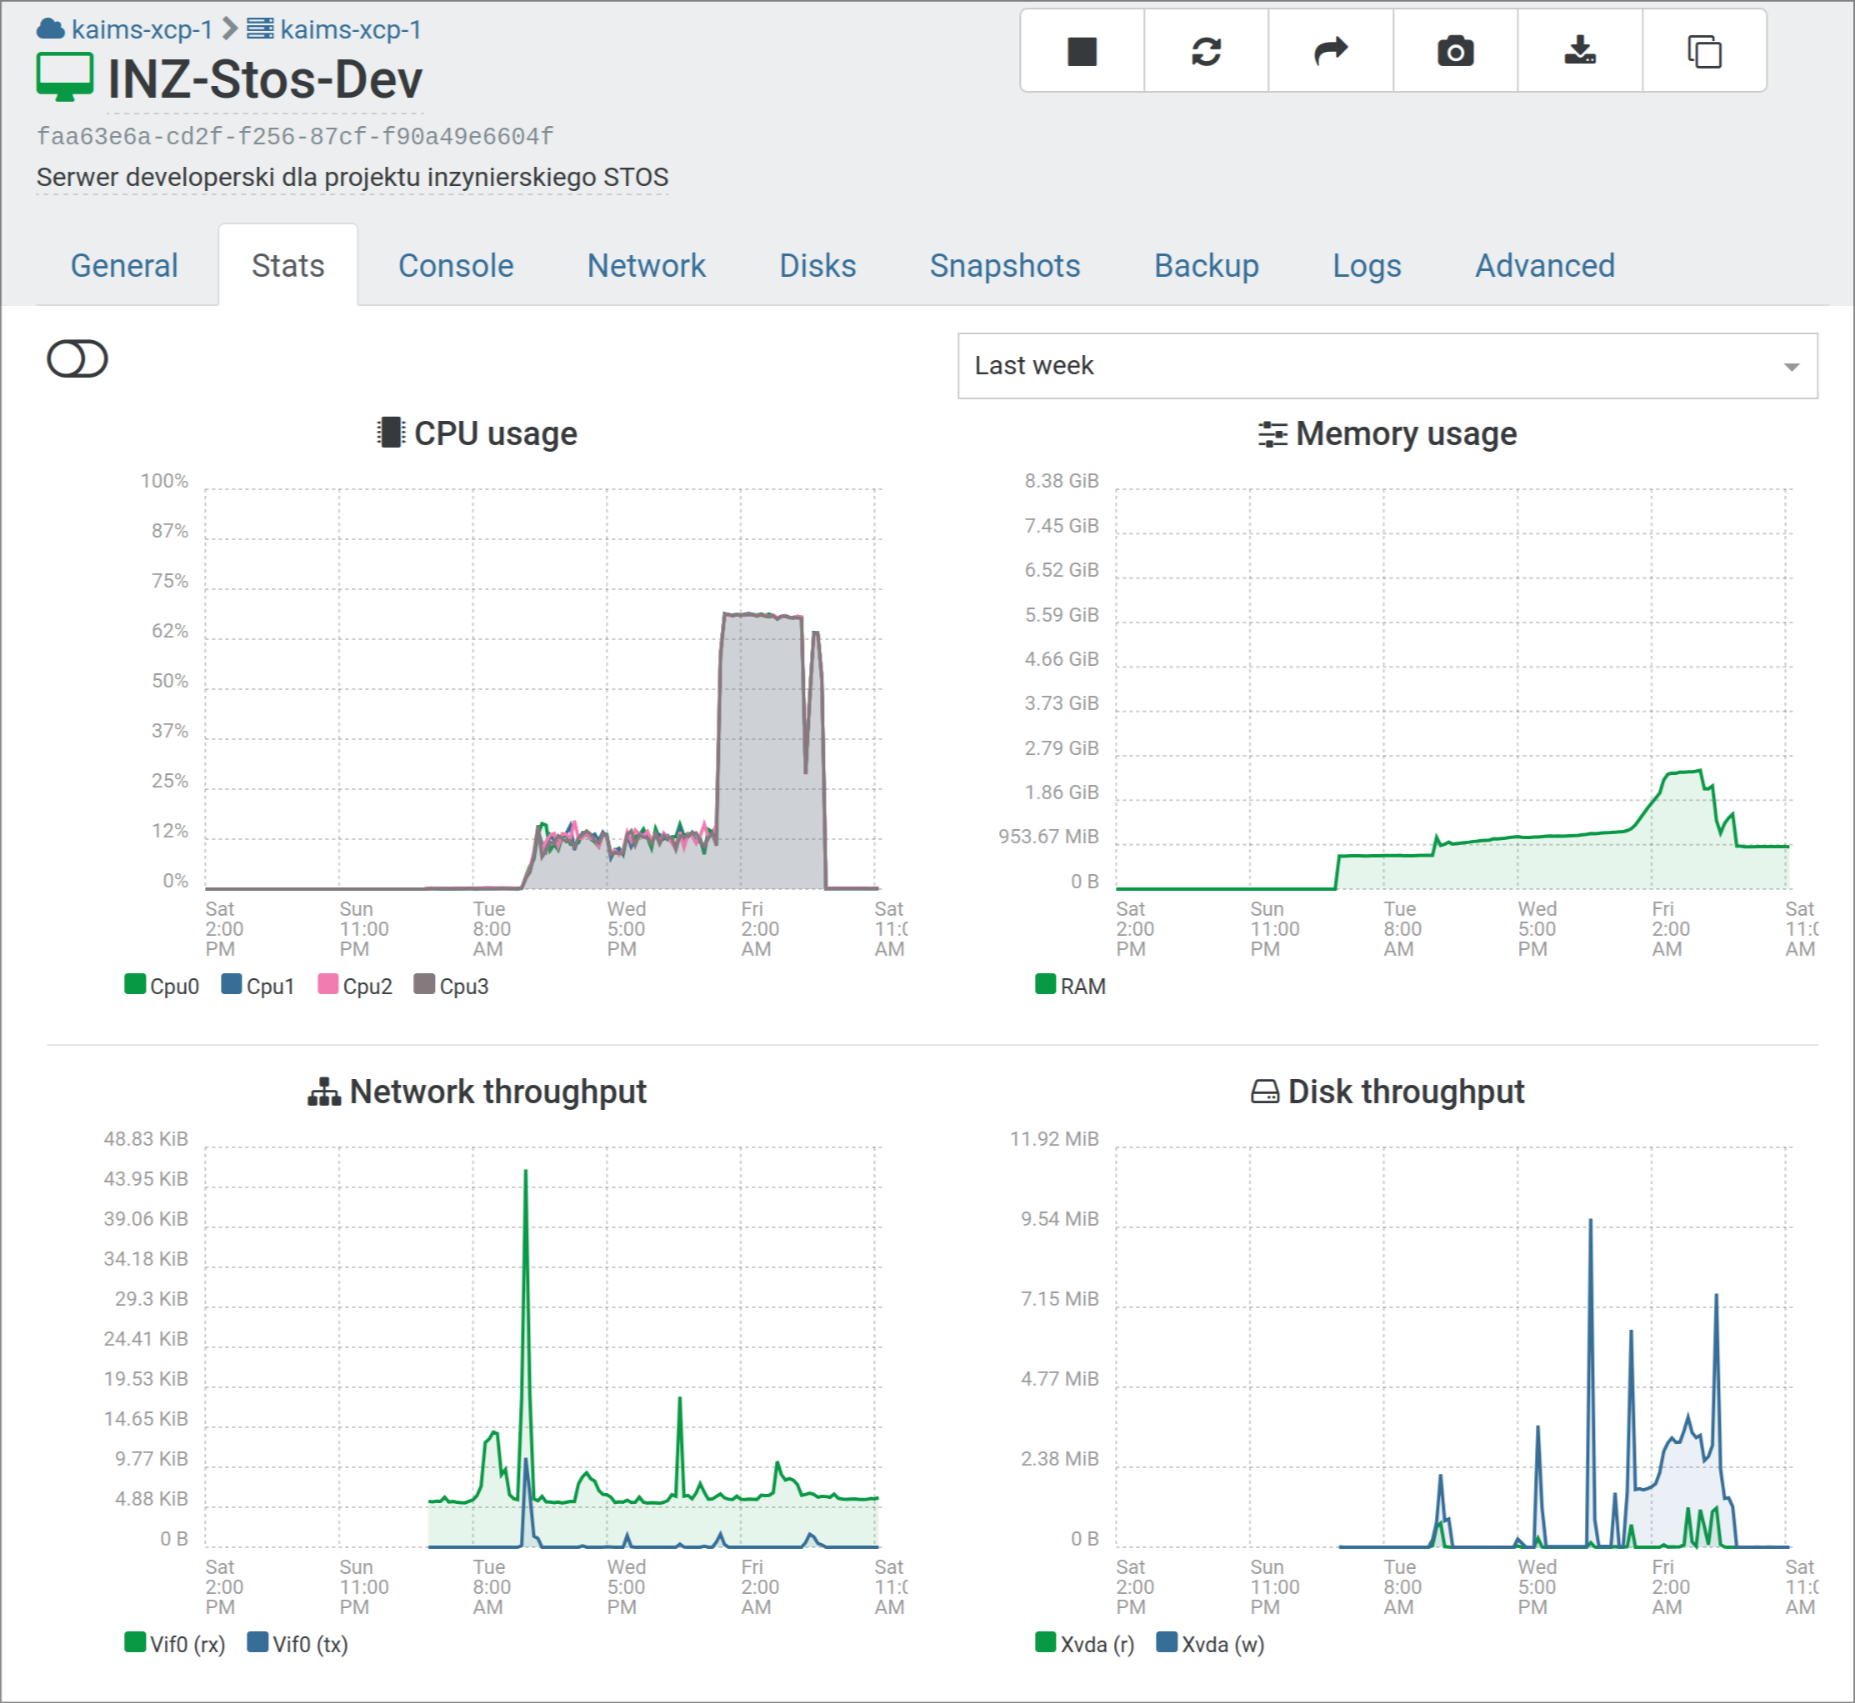
\includegraphics{img/4/xe-dashboard.png}
		}
		\caption[Dashboard Xen Orchestra]{Wizualizacja zasobów sprzętowych zużywanych przez maszynę wirtualną ze środowiskiem testowym systemu STOS widoczna na stronie internetowej udostępnianej przez maszynę Xen Orchestra. Źródło własne.}
		\label{xcpGuest}
	\end{center}
\end{figure}
\subsection{Systemd}
Systemd to pakiet oprogramowania odgrywający rolę menadżera konfiguracji serwisów systemu, nadzorcy startu systemu i~aplikacji monitorującej działanie programów \textit{(demonów)} działających w~tle podczas użytkowania systemu\cite{systemd}. Został on opublikowany 30 marca 2010 i~zyskał większą popularność w~roku 2015, kiedy to większość dystrybucji systemu Linux odbyło migrację z poprzedniego systemu zarządzającego uruchomieniem maszyny, \textit{(SysV Init)}, na systemd. Korzysta z niego również dystrybucja systemu Linux wykorzystana w~maszynach wirtualnych \textit{STOS-dev} i~\textit{STOS} - Debian Bookworm. Uczyniło to systemd naturalnym wyborem w~celu zapewnienia funkcjonalności automatycznego restartu i~monitorowania aplikacji STOS. 
\newline \noindent Aby wykorzystać systemd do zarządzania aplikacją STOS, konieczne było zdefiniowanie własnego pliku konfiguracyjnego opisującego STOS jako serwis w~kontekście systemd (szczegóły implementacyjne opisane zostały w~kolejnym podrozdziale)\cite{systemd-service}. Wykorzystując polecania wbudowane w~pakiet systemd -- \textit{systemctl} i~\textit{journalctl}, możliwe jest proste uruchamianie i~restartowanie serwisu, jak i~monitorowanie deskryptora stderr uruchomionego procesu, co pozwala uprościć zarządzanie aplikacją i~skrypty automatyzujące wdrożenie aplikacji.
\subsection{nix i~\textit{nix-shell}}
Nix to menadżer pakietów, którego oryginalnym autorem jest Eelco Dolstra\cite{nix-repo}. To, co czyni go oryginalnym w~skali wszystkich innych rozwiązań służących do zarządzania pakietami w~systemach z rodziny UNIX \textit{(apt, pacman, homebrew)} to paradygmat konfiguracji -- zamiast imperatywnego podejścia do instalacji pakietów, nix korzysta z podejścia deklaratywnego, które zakłada definiowanie odpowiednich plików konfiguracyjnych opisujących docelowy stan środowiska, bez wskazywania przez użytkownika kroków, jakie należy podjąć, aby doprowadzić do takiego stanu, czym cechuje się podejście imperatywne. Pozwala to na znaczne uproszczenie procesu replikacji środowiska pomiędzy wieloma maszynami, ponieważ wymaga to jedynie udostępnienia wcześniej przygotowanego pliku opisującego stan końcowy środowiska każdej maszynie docelowej i~wywołaniu polecenia \textit{nix-shell} w~celu jego inicjalizacji. 
\newline \noindent Program \textit{nix-shell} jest częścią instalacji samego menadżera pakietów nix. Pozwala on na dynamiczne uruchamianie środowisk powłoki wiersza polecenia na podstawie pliku konfiguracyjnego\cite{nix-shell}. Oprócz definicji samych pakietów, konfiguracja \textit{nix-shell} pozwala również na definiowanie opcji opisujących zachowanie samego środowiska, takich jak stopień izolacji od środowiska będącego jego „rodzicem”, co pozwala na jego efektywną izolację. Dodatkową zaletą jest zwiększenie bezpieczeństwa aplikacji, ponieważ w~przypadku ataku ze strony trzeciej na aplikację, sprawcy mają dostęp tylko do bibliotek i~pakietów niezbędnych do funkcjonowania aplikacji, minimalizując zagrożenie rozprzestrzenienia się potencjalnego ataku.
\newline \noindent Warto nadmienić, że \textit{nixpkgs}, repozytorium pakietów, z którego korzysta nix, jest jednym z największych dostępnych repozytoriów pakietów. Rysunek \ref{wykresRepo} przedstawia zestawienie ilości dostępnych pakietów dla wielu dostępnych repozytoriów -- różne kanały \textit{nixpkgs} posiadają widoczną przewagę na znamienitą większością pozostałych repozytoriów, z wyjątkiem repozytorium \textit{AUR} - Arch User Repository.

\begin{figure}[!h]
	\begin{center}
		\resizebox{0.9\textwidth}{!} {
			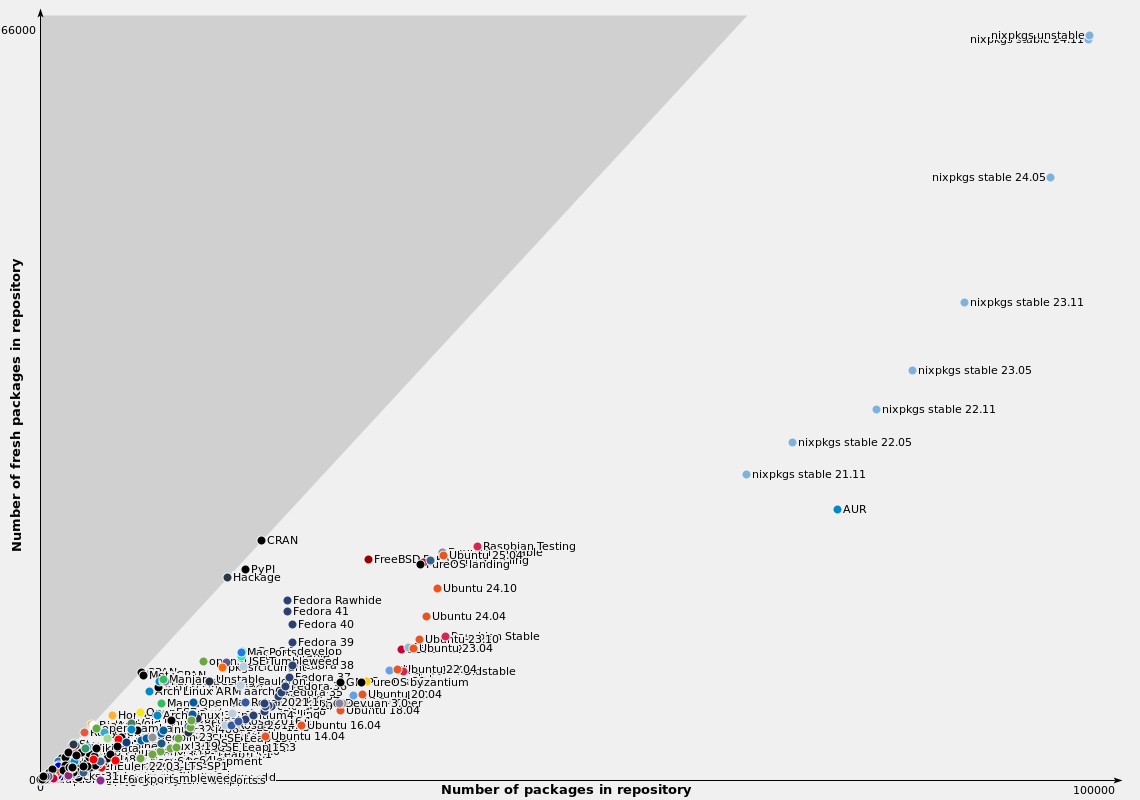
\includegraphics{img/4/repo.png}
		}
		\caption[Ilość aktualnych pakietów i~łączna ilość pakietów w~repozytoriach]{Wykres przedstawiający łączną ilość pakietów i~ilość aktualnych pakietów dla różnych repozytoriów pakietów, stan na 22.11.2024. Źródło: \textit{repology.org}}
		\label{wykresRepo}
	\end{center}
\end{figure}
